%%%%%%%%%%%%%%%%%%%%%%%%%%%%%%%%%%%%%%%%%%%%%%%%%%%%%%%%%%%%%%%%%%%%%%%%%%%%%%%%%%%%%
%%%  EKAW 2016 DC - Modeling, Exploring and Recommending Music in its Complexity  %%%
%%%%%%%%%%%%%%%%%%%%%%%%%%%%%%%%%%%%%%%%%%%%%%%%%%%%%%%%%%%%%%%%%%%%%%%%%%%%%%%%%%%%%

\documentclass{llncs}

\usepackage{url}
\usepackage{graphicx}
\usepackage{xtab}
\usepackage[inline]{enumitem}
\usepackage[title]{appendix}
\DeclareGraphicsExtensions{.png}

%%%%%%%%%%%%%%%%%%%%%%%%%%%%%%%
%%%  Beginning of document  %%%
%%%%%%%%%%%%%%%%%%%%%%%%%%%%%%%

\begin{document}

\title{Modeling, Exploring and Recommending\\ Music in its Complexity}

\author{Pasquale Lisena}
\authorrunning{Lisena} 
\institute{EURECOM, Sophia Antipolis, France \\
\email{pasquale.lisena@eurecom.fr}}

\maketitle

%%%%%%%%%%%%%%%%%%
%%%  Abstract  %%%
%%%%%%%%%%%%%%%%%%

\begin{abstract}
Knowledge models that are currently in-use for describing music metadata are insufficient to express the wealth of complex information about creative works, expressions, performances, publications, authors and performers. In this research, we aim to propose a method for structuring the classical music information coming from different heterogeneous librarian repositories. In particular, we research and implement an appropriate music ontology based on existing models, controlled vocabularies and tools for converting and visualizing the metadata. Moreover, we research how this data can be consumed by end-users, through the development of a web application for exploring the data and a recommendation system that takes advantage of the richness of the data.
\keywords{Ontology, FRBRoo, Musical Metadata, Schema.org, Recommendation}
\end{abstract}

%%%%%%%%%%%%%%%%%%%%%%%%%%%
%%%  Problem Statement  %%%
%%%%%%%%%%%%%%%%%%%%%%%%%%%

\section{Problem Statement}
\label{sec:problem}
Music metadata can be very complex. Let's consider a well-known masterpiece such as Beethoven's \textit{Moonlight Sonata}: structured metadata can describe the music work as composed by the German composer, its scores in the handmade original version or in the Italian transcription or in the different printed editions, the multiple interpretations by pianists and not only, thanks to orchestrations and arrangements. Related to these interpretations, the performances, concerts, recordings, music albums edited on CDs and other media can also be described. Numerous actors are involved in this media production chain: composers, performers with different but well-defined roles, conductors, technicians, etc.

Often, online musical content holders offer a very simplified version of this information, focused on the track as the atomic unit, the artist as the unique carrier of the authorship, and presence in the same album as unique possible relationship between tracks. Beethoven is often not even specified as the ``artist'' of Moonlight Sonata in Spotify or Deezer, while sometimes his name may be displayed near the performer's one, without any distinction between their roles. While a simplified version of the metadata is sometimes enough for commercial purpose, expressing the whole complexity of the music information opens up new possibilities for advanced search, visualization of music influences, and for developing new recommendation strategies for musical applications.

Libraries are used, in contrast, to have much more structured information describing items that are often represented in specialized formats such as MARC\footnote{\url{https://www.loc.gov/marc/}}. The limit of this solution is that developers are tied to these specialized structure. Moreover, following a decentralized policy, each institution hosts data in its repositories, often using a particular dialect of MARC. As result, the music metadata has currently no chances of reconciliation and interconnection. The benefits about moving from MARC to an RDF-based solution consist in the interoperability and the integration among libraries and with third part actors (like publishers and museums), with the possibility of realize a smart federated search thanks to the adoption of common controlled vocabularies \cite{byrne2010strongest}.

This thesis aims to propose a new model for representing music metadata in its full complexity. Music metadata from librarian institution, converted in this model, should then be reconciled and interlinked. Next, we will research, design, implement and evaluate novel applications that use this metadata with the purpose of exploring and recommending music.
% expand these 2 lines ... what are the problems? You just mention the ultimate goals but this is a problem statement section. Don't you want to say a word about the fact that music metadata is spread (decentralized) among multiple repositories ... so that your knowledge model should also come with reconciliation strategies in order to reconcile information and to improve the overall quality of the music metadata?
%PL: updated in the previous paragraph

This research is being developed in the context of the DOREMUS project\footnote{\url{http://www.doremus.org}}~\cite{achichidoremus}, in which three leading cultural institutes in France --- the BnF (Biblioth\`eque Nationale de France), the Philharmonie de Paris and Radio France --- join forces with companies and academic institutions in order to make the music knowledge in their catalogs available and re-usable on the web of data.

%%%%%%%%%%%%%%%%%%%%%%%%%%%%
%%%  Proposed Approach   %%%
%%%%%%%%%%%%%%%%%%%%%%%%%%%%

\section{Proposed Approach}
\label{sec:approach}
Three different challenges represent the ambitious goal of this research thesis.

The first challenge is to find an appropriate ontology model for capturing the richness of music information, taking into account all its components. The data in MARC format from the source institutions will be converted independently in RDF. After that, a reconciliation process should be realized. In particular, \texttt{sameAs} links should be found on the resources from the different institution that describe the same work (or expression, etc.), for letting them finally converge in a unique graphs that contains the whole information at our disposal. This should be realized by identifying the features that let us to point directly a resource (i.e. for a work they could be the title, the author and the catalog number) and comparing them. Moreover, controlled vocabularies must be used for describing specific features (keys, genres, etc.) and disambiguating their values.

The second challenge consists in providing a simplified version of this structured metadata, tailored to be consumed by search engines and third-part applications. Because of its central role in this field, we will provide mappings of this ontology into Schema.org\footnote{\url{http://schema.org}}. Some research questions are:
\begin{enumerate*}
\item{\textit{which information should be presented in this simplified version and which one is considered too complex?}}
\item{\textit{which methods should be used for realizing this simplification?}}
\end{enumerate*}

Finally, our aim is to demonstrate the benefits that these data can produce once they are consumed and displayed to the end-user. We consider taking the user in account as a crucial requirement for the design of these systems. In this context, an application will be developed that consists in two parts. Firstly, an exploratory search engine for musical data will be designed and developed. \textit{Can the knowledge model simplification operated in the second challenge be used to improve the user experience? How complex concepts and relationship should be displayed to the end-user?} On top of the exploratory interface, we will build a recommendation engine. \textit{Are the recommendation systems currently used for music still valid for this complexity? Is the rich model better then the simplified (Schema.org-based) one for feeding the recommendation? Do different user profiles (the student, the expert, the music amateur) require different recommendations?}

%%%%%%%%%%%%%%%%%%%%%%%%%
%%% State of the Art  %%%
%%%%%%%%%%%%%%%%%%%%%%%%%

\section{State of the art}
\label{sec:state-art}

\subsection{Musical data representation}
The description of music is historically connected to catalog information models, among which FRBR is one of the most popular. This model describes a literary entity at 4 levels: Works, Expression, Manifestation and Item. FRBR and CIDOC-CRM, an ontology for describing bibliographic and museum information, have been harmonized in the FRBRoo ontology for describing arts \cite{doerr2008frbroo}. This model consider events as an essential part of the cultural entity, that exists only in the combination of the Work (the author's intention) that is realised into an Expression through an Event creation. This triplet Work-Expression-Event is a common pattern in FRBRoo.

Built on top of FRBR, the Music Ontology proposes a model in three levels: the first for editorial information (title, composer, year, album), the second for events (composition, performance, recording) and the third for complex event decomposition (fragment and instants) \cite{raimond2007music}. In \cite{song2009music}, an ontology named COMUS (Context-based Music Recommendation) is presented, with the specific purpose of structure data for make them fit in a recommendation system, in which concepts as mood, genre and situation gain a strong importance.

Different experiences about converting data from MARC to RDF have been explored\footnote{\url{https://github.com/search?q=marc2rdf}}. The \textit{datos.bne.es} project has developed MARiMbA \cite{greenberg2013datos}, a software for the conversion of MARC data from the Spanish National Library in RDF, using the FRBR model. Moreover, it manages also the following steps: interlinking data, loading data in a triple store, providing a simple visualization of the data.

\subsection{Music recommendation}
Music recommendation is an active and popular research field. Most of the important actors in online music (Spotify, Deezer, Last.fm, YouTube) provide some sort of recommendations to keep their users engaged in their platform. Having generally a large user base, those platforms often make use of collaborative recommendation algorithms. 

The need to discover novelty in results (that coincides with the user's need for listening new songs) requires the use of different approaches that the ones generally used for simple product recommendation. Among them, we can cite the use of the Long Tail curve for also including less popular works in recommendation \cite{celma2009music} and the prediction of latent factors for the new items inserted in the database \cite{van2013deep}.

A feature-combination hybrid approach is presented in \cite{ostuni2015soundrec}: the datasets of Last.fm and Songfacts.com are semantically enriched through external graphs (DBpedia and WordNet). This content-based features are combined with collaborative information in order to provide better results in terms of both accuracy and novelty.

The approaches completely based on the knowledge of the model are less common. An example is the use of the information about the location and period of the composition (or of the composer) for realize a recommendation system driven by the places of interests nearby the user \cite{kaminskas2012knowledge}. 

A richer model opens up new ways to design a recommendation system. A precisely structured information allows you to select different salient features for the knowledge-based recommendation and assign them a scale of finer weights. To this we can add the ability to create playlists based each time on a different property (the genre, the historical period, the location, a musical instrument). In addition, this knowledge-base techniques can be improved and corrected by the collaborative ones.
% good state-of-the art section ... but, how do you conclude it? What is still not done? Where will you differentiate? What do you take from this related work and what will you aim to improve?
% PL edit done

%%%%%%%%%%%%%%%%%%%%%%
%%%  Methodology   %%%
%%%%%%%%%%%%%%%%%%%%%%

\section{Methodology}
\label{sec:methodology}
Different parts of this thesis are currently carried out in parallel, in order to have in mind the final goals during the development of the various strategies.

\subsection{DOREMUS Ontology}
The DOREMUS ontology \cite{choffe2016doremus} is being developed as an extension of the FRBRoo model. The choice about designing a new ontology on top of FRBRoo comes from two main reasons: a fine granularity of description (suitable for  the complexity of music) granted by the triplet pattern, and the possibility to interoperate with information systems dealing with any kind of cultural data. A modelling group, to which experts of music catalogs and of the web of data are part, is currently working on the ontology. The DOREMUS model\footnote{\url{https://github.com/DOREMUS-ANR/doremus-ontology}} contains today 149 classes and 346 properties.

\subsection{Controlled vocabularies}
In addition to the core DOREMUS ontology, using various controlled vocabularies enables to refer to concepts in an unambiguous way. Different kind of vocabularies are needed for describing music: some are already available on the web (like media of performance\footnote{\url{http://iflastandards.info/ns/unimarc/terms/mop/}} or musical genres\footnote{\url{http://iflastandards.info/ns/unimarc/terms/fom/}}, other not existing at all (like the derivation types).
Not all of them are published in a suitable format for the Web of Data, and there is no often little interconnection between vocabularies. Our effort is to provide a SKOS controlled vocabulary for each of them, with appropriate relationships and mappings between the different sources.
\begin{enumerate}
\item{Persons and corporate bodies: ISNI\footnote{\url{http://www.isni.org/}}}
\item{Ethnic groups: RAMEAU\footnote{\url{http://rameau.bnf.fr/}}}
\item{Functions: UNIMARC\footnote{\url{http://id.loc.gov/vocabulary/relators.html}}, RDA\footnote{\url{http://web.library.yale.edu/cataloging/music/relationshipdesgi}}}
\item{Musical genres: IAML\footnote{\url{http://www.iaml.info/}}, RAMEAU}
\item{Medium of performance: MIMO\footnote{\url{http://www.mimo-db.eu/}}, IAML, RAMEAU}
\item{Keys: MusicOntology\footnote{\url{http://musicontology.com/}}}
\item{Derivation type: not existing}
\end{enumerate}

\subsection{Simplification through Schema.org.}
%TODO If our paper is accepted at EKAW, can we cite it?
%RT: add already the bib ref, with the mention "submitted to ..."
%PL: I did it anyway (considering it a poster paper)

Schema.org contains different types for describing music: CreativeWork, MusicComposition, MusicRecording, MusicGroup, etc. Passing from FRBRoo to the Schema.org model means finding a strategy for mapping the concept expressed in a complex ontology to a simpler one. We have proposed a method composed of a series of recipes that enables to perform this operation based on the observation of the graph \cite{lisena2016mapping}. Figure \ref{fig:beethoven-mapping} shows a mapping of Beethoven's \textit{Sonata ``Quasi una Fantasia"} as result of the selection of the most important classes (in the figure, the yellow ones), the individuation of the relative Schema.org types through similarity criteria, the iterative extension to their properties until covering the whole graph. 
%TODO: add an example (the one from the EKAW paper) of the complex model and the simplified one if you have enough space
%PL double check if it is understandable

\begin{figure}
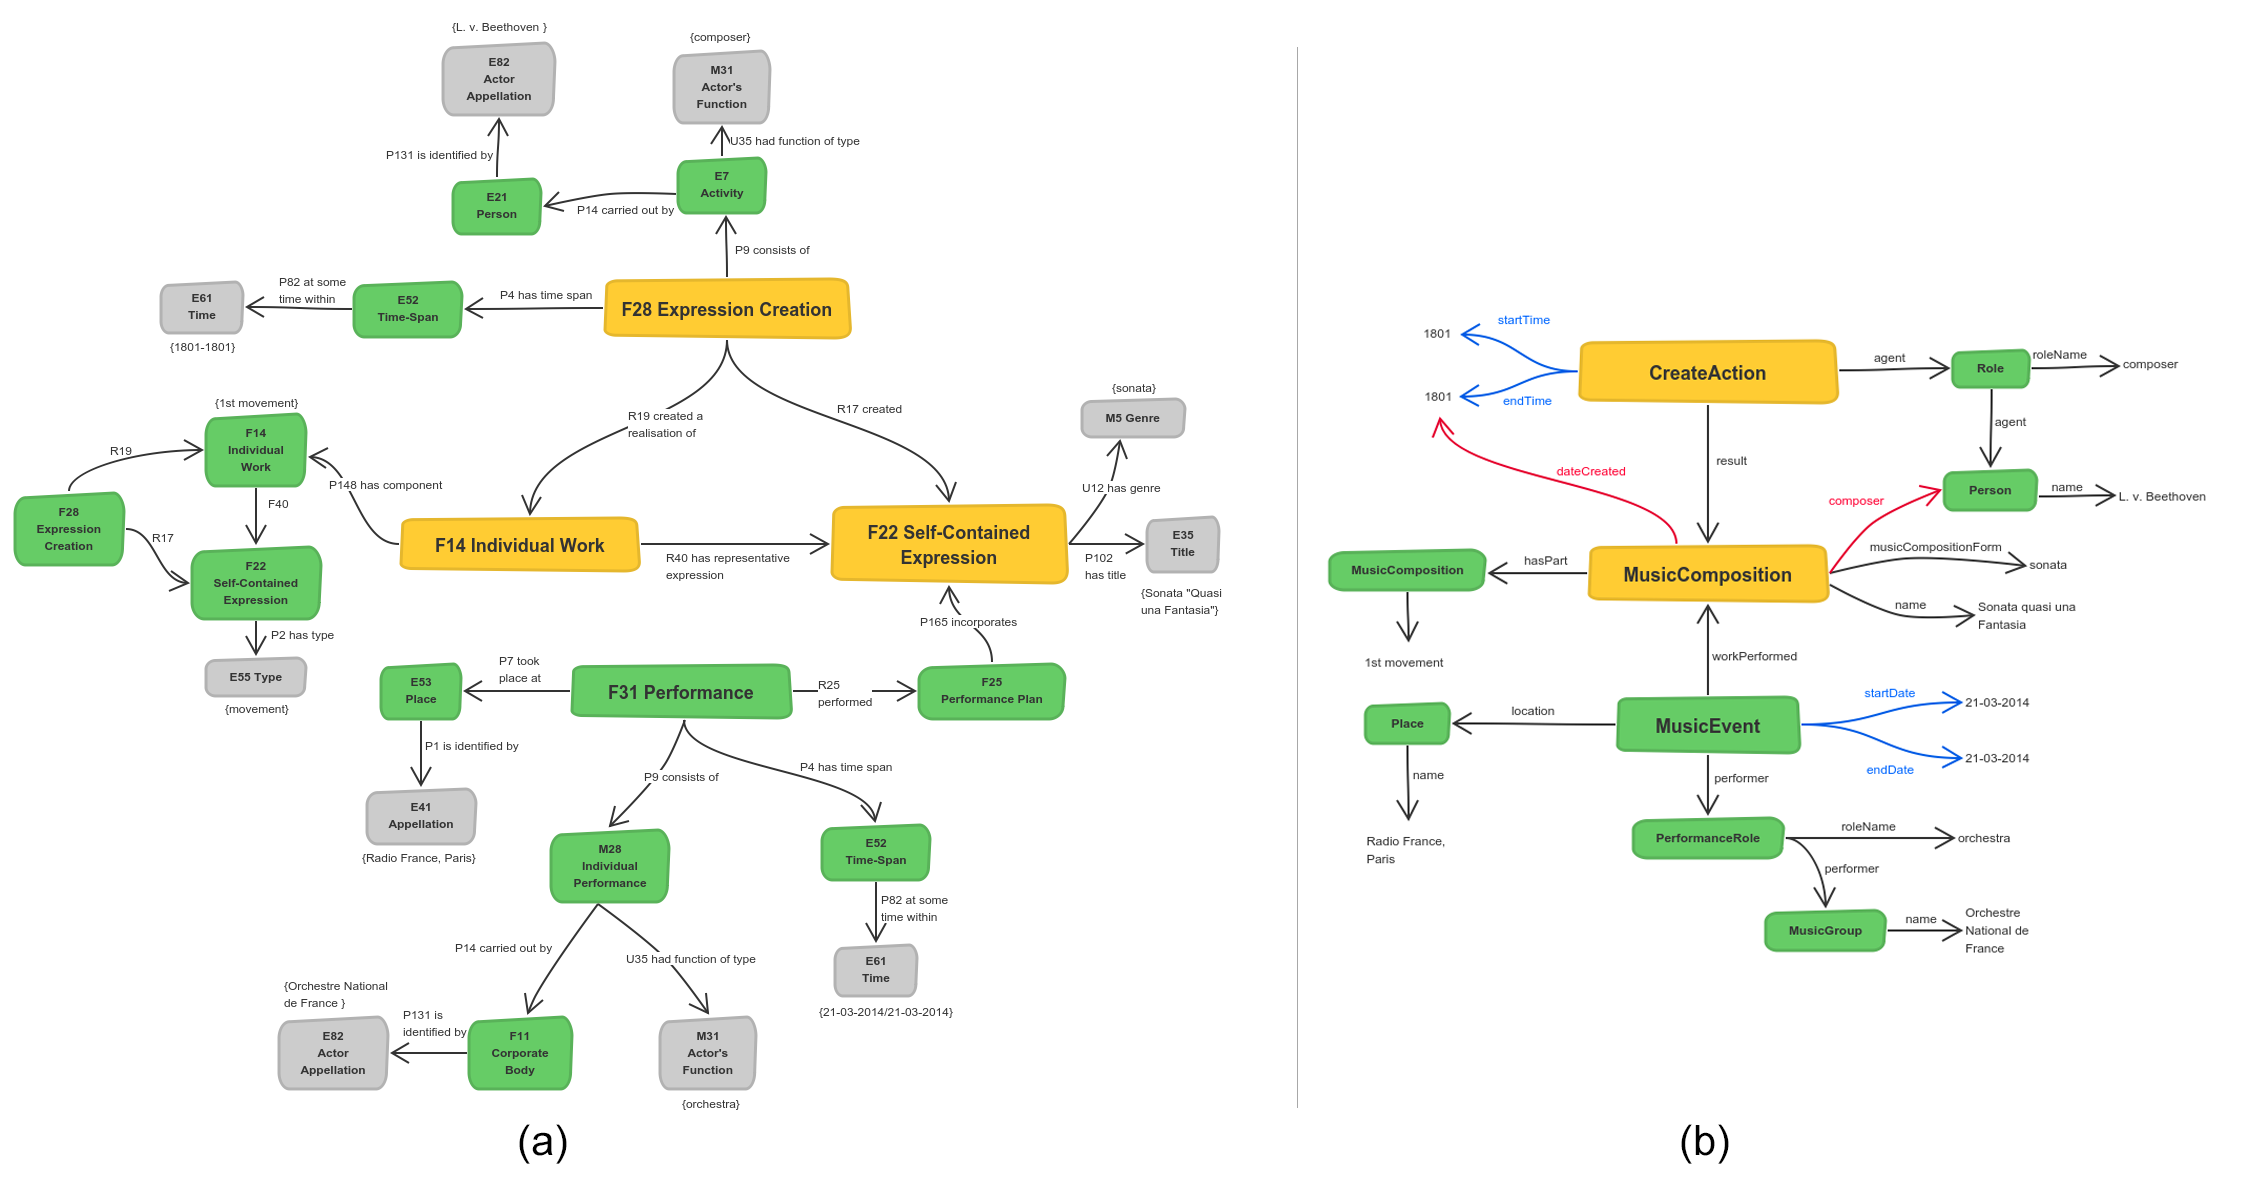
\includegraphics[width=12cm]{img/Beethoven-mapping.png}
\centering
\caption{Graph of Beethoven's \textit{Sonata ``Quasi una Fantasia"} described through the DOREMUS ontology (a) and simplified with our recipe to Schema.org  (b).}
\label{fig:beethoven-mapping}
\end{figure}


\subsection{Recommendation} Our starting point for the study of a suitable algorithm for recommendation consists in two human-made collections: playlists from RadioFrance and concert programs from Philharmonie de Paris. While the latter can reveal very strong connection between works (so that they are played in the same concert, probably with the same casting), in the former the logical succession (redacted by experts for an amateur public, sometimes inside thematic radio programs) should contain also a novelty factor.

In parallel to these collections, we can consider the results of the recommendations from leading music providers. In this context, we realized the ARyTREx web app\footnote{Experiment realized by Eva Fern\a'andez-Mar\a'in during the realization of her master thesis (\url{https://github.com/fernanev/ARyTREx}).}, which uses the API from Spotify and Last.fm for showing different recommendation paths, collecting the metadata of the included tracks. 

A goal will be to identify which features are the most important in the recommendation. The DOREMUS ontology itself will be able to describe the results, making available to the web a set of thematic playlists.

Programs, playlists and third-parts recommendation results will play a key role in the evaluation of the algorithm, that can be iteratively corrected by the comparison between its output and these collections. Precision and recall metrics will be used to measure this comparison.

%TODO: if you have space, I think you could be more verbose here ... talk about Eva's work in simulating traces for getting recommendations. Another challenge is how to model / represent those playlists? How will you evaluate the accuracy of those recommendations, using which evaluation protocol, which metrics?
%PL the evaluation part could be improved (I'm reading a paper on this)

%%%%%%%%%%%%%%%%%%%%%%%%%%%%%%
%%%  Preliminary results   %%%
%%%%%%%%%%%%%%%%%%%%%%%%%%%%%%

\section{Preliminary results}
\label{sec:results}
Since the start of the project, some results have been achieved. We have developed a prototype \textsc{marc2rdf} conversion tool and a prototype exploration tool named \textsc{Overture}, both as open source softwares~\cite{lisena2016exploring}. 

\subsection{Data conversion}
\textsc{marc2rdf}\footnote{\url{https://github.com/DOREMUS-ANR/marc2rdf}} is an open source prototype for converting the bibliographic records from UNIMARC and INTERMARC to an RDF graph following the DOREMUS model. The conversion relies on explicit expert-defined transfer rules (or mappings), that define for each property/class in the DOREMUS ontology where to find the relative information in the MARC file. The software contains also a \textit{string2uri} component, inspired by the Datalift platform \cite{scharffe2012enabling}, that performs an automatic mapping of string literals to URIs coming from controlled vocabularies.

\subsection{Data exploration}
First studies about the exploratory application have been started. A prototype of an exploratory web application named \textsc{Overture} (Ontology-driVen Exploration and Recommendation of mUsical REcords)\footnote{\url{https://github.com/DOREMUS-ANR/overture}} is under development. The challenge is in giving to the final user a complete vision on the data of each work, performance, score, recording and letting him/her to understand how they are connected to each other. At the same time, the application must have an easy and pleasant user experience. 
%Figure \ref{fig:overture-gui} shows a preliminary proposal for the GUI. 
Recommendation will be present in the next versions of the application.

%\begin{figure}
%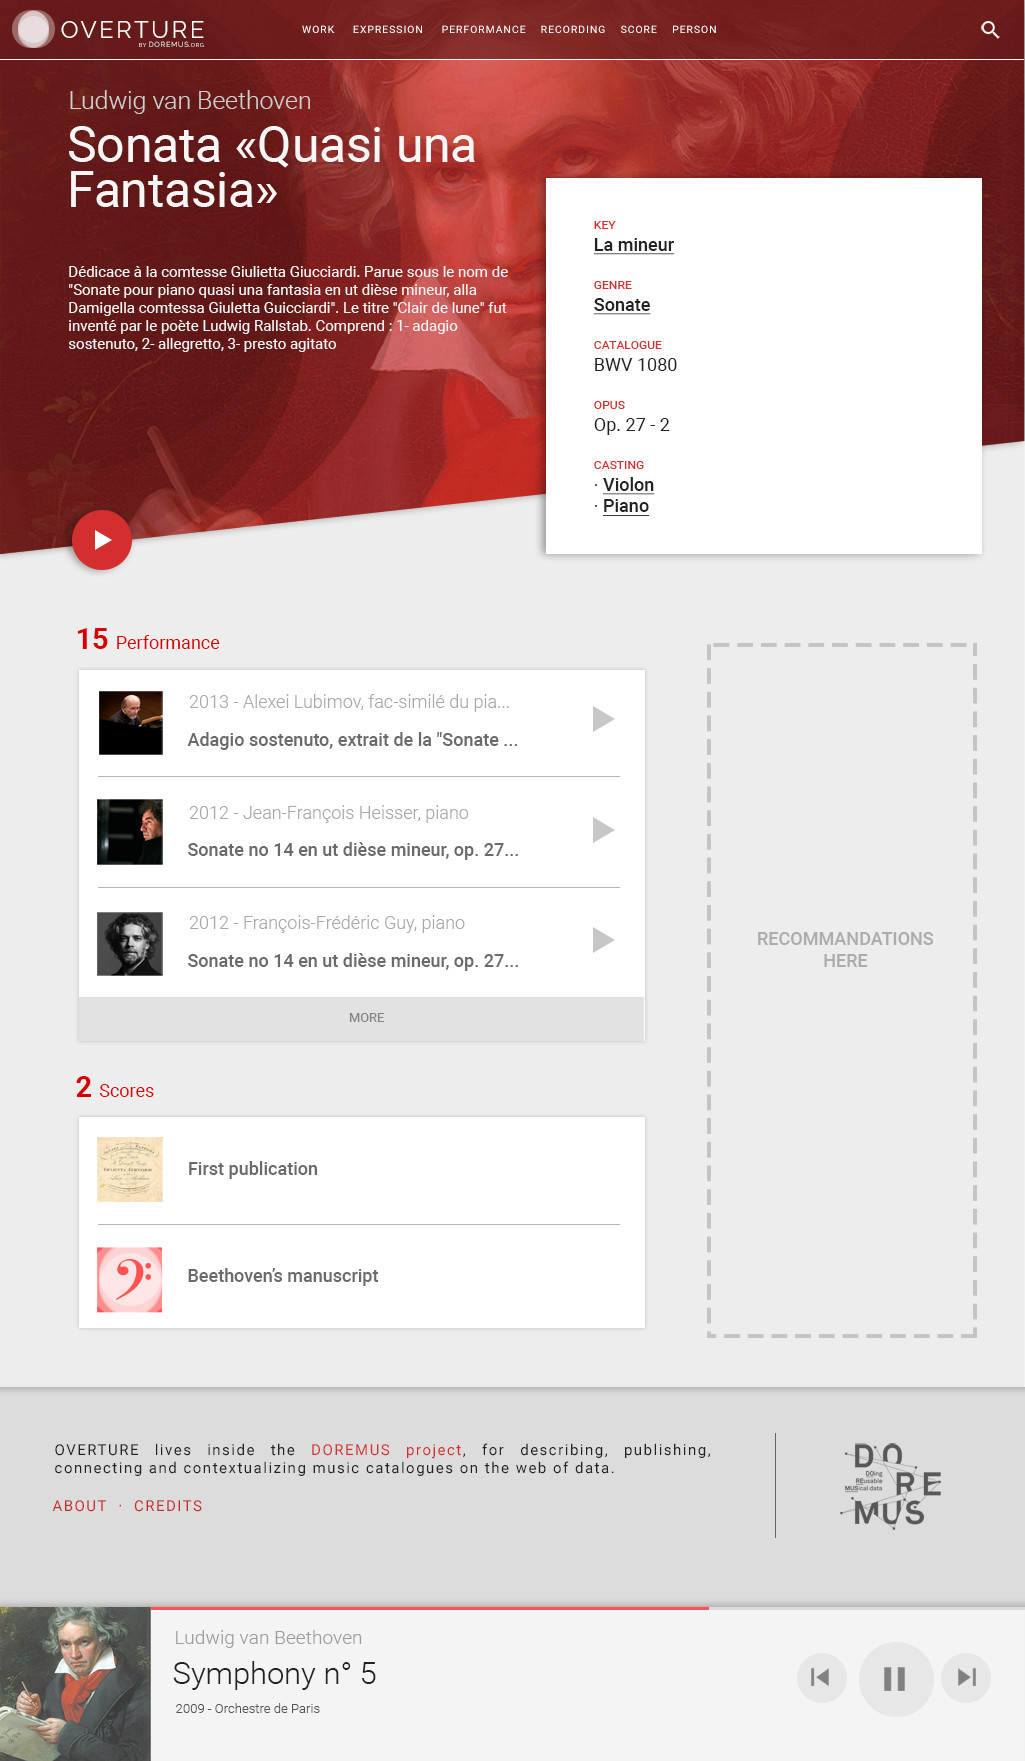
\includegraphics[width=8cm]{img/Expression.jpg}
%\centering
%\caption{A first design of the exploratory interface.}
%\label{fig:overture-gui}
%\end{figure}

A first version of the exploratory interface is available at \url{http://overture.doremus.org}.

%%%%%%%%%%%%%%%%%%%%%%%%%%%%%%%%%%%%
%%%  Conclusion and Future Work  %%%
%%%%%%%%%%%%%%%%%%%%%%%%%%%%%%%%%%%%

\section{Conclusion and Future Work}
\label{sec:conclusion}
Representing the information about classical music is a complex activity, that involves different sub tasks. During this research, we want to express the musical metadata from their current MARC format in a suitable ontology that can preserve their complexity. From that, a simplification through Schema.org will guide the realization of a exploratory interface, while the richness of the model will help the realization of a recommendation system.

A full publication of all DOREMUS data (ontology, vocabularies, metadata) is foreseen shortly after the time of writing. A SPARQL endpoint is already online\footnote{\url{data.doremus.org/sparql}} with some data (a thematic collection of work from Beethoven and from Dutilleux). Disambiguation of data and interlinking between resources should be performed in the context of controlled vocabularies. Also the data coming from the conversion of partner institutions should be interlinked, so that different descriptions of the same work go enriching each other. Then, this research will go deep in the data presentation in OVERTURE and in the implementation of the recommendation system.

\section*{Acknowledgments}
I would like to express my thanks to my supervisor Rapha\"el Troncy for his ongoing support in writing this thesis. This work has been partially supported by the French National Research Agency (ANR) within the DOREMUS Project, under grant number ANR-14-CE24-0020.

% ---- Bibliography ----
\bibliographystyle{abbrv}
\bibliography{bib-doremus}

\end{document}